%========================
% Document class and theme
%========================
\documentclass[8pt]{beamer}
\usetheme[progressbar=frametitle]{metropolis}
\setbeamersize{text margin left=10mm, text margin right=10mm}
\usepackage{appendixnumberbeamer} % appendix slide numbering
\setbeamertemplate{theorems}[numbered]

%========================
% Core packages
%========================
\usepackage{amsmath, amsfonts, amssymb, amsthm} % math + theorems
\usepackage{booktabs}        % professional tables
\usepackage{hyperref}        % hyperlinks
\usepackage{xcolor}          % colors
\usepackage{xspace}          % spacing for custom commands

%========================
% Algorithms
%========================
\usepackage{algorithm}
\usepackage{algpseudocode}
\newtheorem{proposition}{Proposition}
\usepackage{bbm}

%========================
% Plots and TikZ
%========================
\usepackage{pgfplots}
\usepgfplotslibrary{dateplot}
\usepackage{tikz}
\usetikzlibrary{positioning}

%========================
% Listings (code)
%========================
\usepackage{listings}
\lstset{
    basicstyle=\ttfamily\small,
    breaklines=true,
    numbers=left,
    numberstyle=\tiny
}

% R style
\lstdefinelanguage{R}{
  morekeywords={TRUE,FALSE},
  deletekeywords={data,frame,length,as,character},
  otherkeywords={0,1,2,3,4,5,6,7,8,9},
  keywordstyle=\color{blue},
  commentstyle=\color{DarkGreen},
  stringstyle=\color{DarkGreen},
  basicstyle=\ttfamily\small
}

% Python style
\lstdefinelanguage{PythonCustom}{
  language=Python,
  keywordstyle=\color{blue},
  commentstyle=\color{gray},
  stringstyle=\color{red},
  basicstyle=\ttfamily\small
}

%========================
% Custom commands
%========================
\newcommand{\themename}{\textbf{\textsc{metropolis}}\xspace}

%========================
% Custom footline
%========================
\setbeamertemplate{footline}
{%
  \leavevmode%
  \hbox{%
  \begin{beamercolorbox}[wd=.35\paperwidth,ht=2.5ex,dp=1.5ex,center]{author in head/foot}%
    \usebeamerfont{author in head/foot}\insertshortauthor
  \end{beamercolorbox}%
  \begin{beamercolorbox}[wd=.3\paperwidth,ht=2.5ex,dp=1ex,center]{title in head/foot}%
    \usebeamerfont{title in head/foot}\insertshorttitle
  \end{beamercolorbox}%
  \begin{beamercolorbox}[wd=.3\paperwidth,ht=2.5ex,dp=1ex,right]{date in head/foot}%
    \usebeamerfont{date in head/foot}\insertframenumber{} / \inserttotalframenumber
  \end{beamercolorbox}}%
  \vskip0pt%
}

%========================
% Beamer tweaks
%========================
\setbeamertemplate{navigation symbols}{} % remove default navigation symbols


%%%%%%%%%%%%%%%%%%%%%%%%%%%%%%%%%%%%%%%%%%%%%%%%%%%%%%%%%%%%%%%%%%%%
%%%%%%%%%%%%%%%%%%%%%%%%%%%%%%%%%%%%%%%%%%%%%%%%%%%%%%%%%%%%%%%%%%%%
% AQUI SE DEFINEN LAS IMAGENES PARA UTILIZAR DESPUES
%\pgfdeclareimage[interpolate=true, height=7cm,width=16cm]{halton-points}{halton-points}
%\pgfdeclareimage[interpolate=true, height=3cm, width =4cm]
%{serie-petroleo-reducido}{serie-petroleo-reducido}
%\pgfdeclareimage[interpolate=true, height=3cm, width =4cm]{rectangle-triangle}{rectangle-triangle}
%\pgfdeclareimage[interpolate=true, height=3cm, width =4cm]{any-angle}{any-angle}
%\pgfdeclareimage[interpolate=true, height=3cm, width =4cm]{Pythagoras}{Pythagoras}


\title{Chapter 2 - Simulating Statistical Models}
\subtitle{Markov Chains on a Continuous State Space.}
\author{Prof. Alex Alvarez, Ali Raisolsadat}
\institute{School of Mathematical and Computational Sciences \\ University of Prince Edward Island}
\date{} % leave empty or add \today
%\title[Stat 4110]{Stat 4110 Statistical Simulation}
%\subtitle{}
%\author[University of Prince Edward Island]{School of Mathematical and Computational Sciences \\ University of Prince Edward Island}

%========================
% Begin document
%========================
\begin{document}

%-------------------
% Title frame
%-------------------
\maketitle

%-------------------
% Slide 1: Markov Chains on Different State Spaces
%-------------------
\begin{frame}{Markov Chains on Different State Spaces}
\textbf{Finite state space:}  
So far we considered Markov chains with  
\begin{equation*}
S = \{1,2,\ldots, M\}
\end{equation*}

\textbf{Beyond finite:}  
Markov chains can also take values in more general spaces, such as  
\begin{equation*}
S = \mathbb{R}^d
\end{equation*}

In this case, instead of a transition \textbf{matrix}, we will need a 
transition \textbf{density}.
\end{frame}

%-------------------
% Slide 2: Transition Density
%-------------------
\begin{frame}{Transition Density}
A \textbf{transition density} is a function 
\begin{equation*}
p:\mathbb{R}^d \times \mathbb{R}^d \to \mathbb{R}
\end{equation*} 
such that:
\begin{enumerate}
	\item $p(x,y) \geq 0$ for all $x,y \in \mathbb{R}^d$.
	\item $\displaystyle \int_{\mathbb{R}^d} p(x,y)\,dy = 1 \quad \forall x \in \mathbb{R}^d$.
\end{enumerate}

\vspace{3mm}

The interpretation of this definition is that $x$ plays the role of the 
current state of the Markov Chain, so for a fixed value of $x$, the function $g(y)=f(x,y)$ is the density function of the random variable $Y$ representing the next state of the Markov Chain.
\end{frame}

%-------------------
% Slide 2: Example - Gaussian Markov Chain
%-------------------
\begin{frame}{Example: Gaussian Markov Chain}
\textbf{Example 2.29 from the Textbook:}  
Let $X_0 = 0$ and define
\begin{equation*}
X_j = \tfrac{1}{2} X_{j-1} + \varepsilon_j, 
\quad \varepsilon_j \sim N(0,1) \ \text{i.i.d.}
\end{equation*}

\vspace{3mm}

\textbf{Observation:}  
The sequence $X_0, X_1, X_2, \ldots$ is a Markov chain with state space $S=\mathbb{R}$.

\vspace{3mm}

\textbf{Conditional law:}  
Given $X_{j-1}=x$, we have
\begin{equation*}
X_j = \tfrac{x}{2} + \varepsilon_j 
\;\;\sim\;\; N\!\left(\tfrac{x}{2},\, 1\right)
\end{equation*}

\vspace{3mm}

\textbf{Transition density:}
\begin{equation*}
p(x,y) = \frac{1}{\sqrt{2\pi}} 
\exp\!\Bigg(-\tfrac{1}{2}\,(y - x/2)^2 \Bigg),
\quad x,y \in \mathbb{R}
\end{equation*}
\end{frame}

%-------------------
% Slide 4: Generation of Markov Chain Paths (Continuous State Space)
%-------------------
\begin{frame}{Generation of Markov Chain Paths (Continuous State Space)}
\begin{algorithm}[H]
\caption{Simulating a Markov Chain Path}
\begin{algorithmic}[1]
\State Generate $X_0$ according to the initial distribution
\For{$i = 1$ to $n-1$}
    \State Generate $X_i \in S$ according to the density
    \[
    g(y) = p(X_{i-1}, y)
    \]
\EndFor
\State \Return $(X_0, X_1, \ldots, X_n)$
\end{algorithmic}
\end{algorithm}
\end{frame}

%-------------------
% Slide 5: Generation of Markov Chain Paths (continuous stat space)
%-------------------
\begin{frame}{Example: Markov Chain Path}
\centering
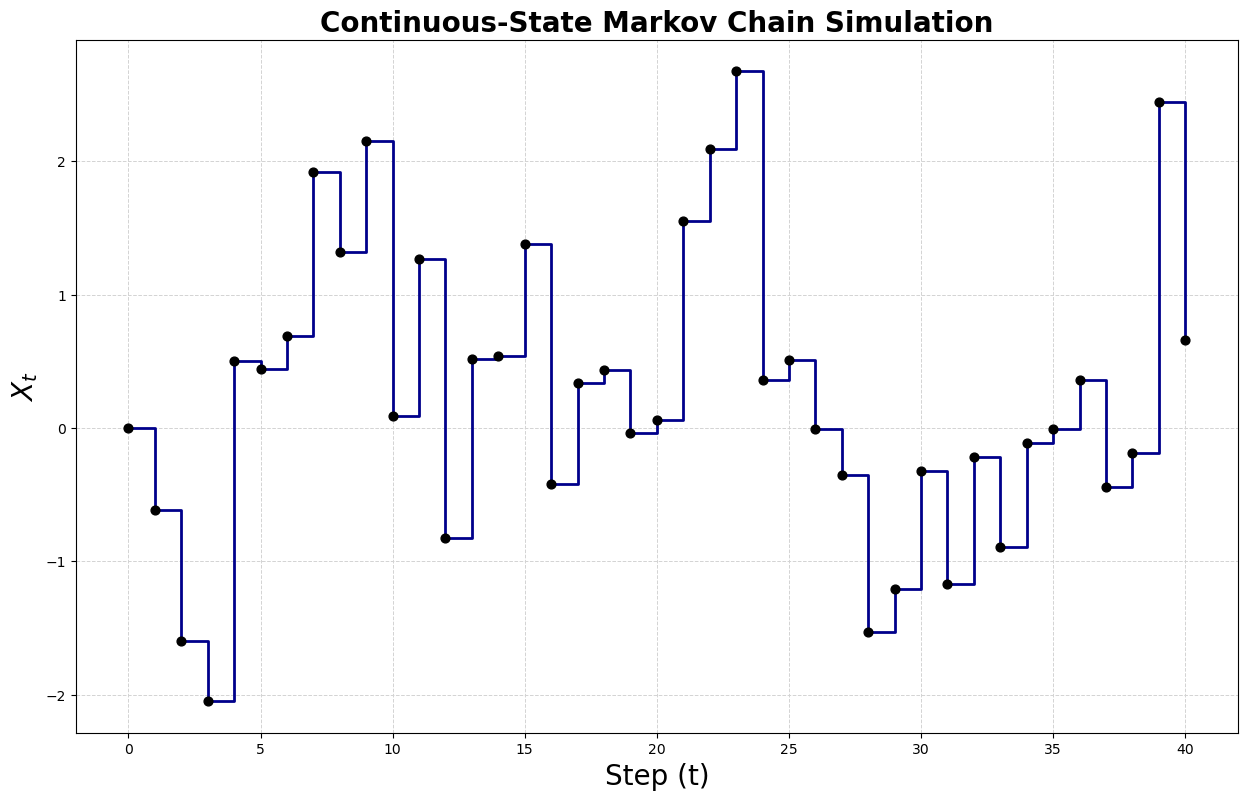
\includegraphics[width=0.9\textwidth]{chapter2-part3-plot1.png}

\vspace{3mm}
\textbf{Simulated trajectory of a continuous state space Markov Chain with $n=40$ with transition density $
p(x,y) = \frac{1}{\sqrt{2\pi}} 
\exp\!\Bigg(-\tfrac{1}{2}\,(y - x/2)^2 \Bigg),
\quad x,y \in \mathbb{R}
$.}
\end{frame}

%-------------------
% Slide 6: Example - Uniform Transition Density
%-------------------
\begin{frame}{Example: Uniform Transition Density}
\textbf{Example (from Homework):}  
Let $X_0 = 0$ and define the transition density
\begin{equation*}
p(x,y) = \tfrac{1}{2} \, \mathbbm{1}_{[x-1,\,x+1]}(y), 
\quad x,y \in \mathbb{R}
\end{equation*}

\vspace{3mm}

\textbf{Note:} The indicator function $\mathbbm{1}_A$ is defined as
\begin{equation*}
\mathbbm{1}_A(y) =
\begin{cases}
1, & \text{if } y \in A, \\[2mm]
0, & \text{if } y \notin A.
\end{cases}
\end{equation*}

\textbf{Observation:}  
The sequence $X_0, X_1, X_2, \ldots$ is a Markov chain with state space $S=\mathbb{R}$.

\textbf{Conditional law:}  
Given $X_{j-1} = x$, we have
\begin{equation*}
X_j \;\sim\; \text{Uniform}(x-1, \, x+1)
\end{equation*}

\textbf{Transition density:}
\begin{equation*}
p(x,y) =
\begin{cases}
\dfrac{1}{2}, & y \in [x-1,\,x+1], \\[2mm]
0, & \text{otherwise}.
\end{cases}
\end{equation*}
\end{frame}


%-------------------
% Slide 7: Stationary Distributions - Intuition & Example
%-------------------
\begin{frame}{Stationary Distribution in Continuous State Spaces}
For Markov chains with a continuous state space, we also have the notion of a 
\textbf{stationary distribution}.

\vspace{3mm}

A probability density $\pi: \mathbb{R}^d \to [0,\infty)$ is called a 
\textbf{stationary density} for a Markov chain with transition density $p$ if it satisfies
\[
\int_{\mathbb{R}^d} \pi(x)\,p(x,y)\,dx \;=\; \pi(y),
\quad \forall \, y \in \mathbb{R}^d.
\]

\end{frame}

%-------------------
% Slide 8: Stationary Distributions - Intuition & Example
%-------------------
\begin{frame}{Stationary Distributions - Intuition \& Example}

\textbf{Intuition:}  
A stationary density $\pi$ is an \alert{equilibrium law} for the Markov chain:
\begin{itemize}
    \item If $X_n \sim \pi$, then $X_{n+1} \sim \pi$ as well.
    \item The distribution is \textbf{invariant} under the dynamics of the chain.
    \item In the long run, many Markov chains converge to their stationary distribution,
    regardless of the starting point.
\end{itemize}

\vspace{3mm}

\textbf{Example (Gaussian AR(1) Chain):}  
\[
X_j = \tfrac{1}{2} X_{j-1} + \varepsilon_j, 
\quad \varepsilon_j \sim N(0,1).
\]

\begin{itemize}
    \item This chain has a stationary distribution:
    \[
    \pi \;\sim\; N\!\Big(0, \tfrac{1}{1-(1/2)^2}\Big) 
    = N\!\Big(0,\tfrac{4}{3}\Big).
    \]
    \item \textbf{Interpretation}: After many steps, the state $X_n$ is approximately $N(0,4/3)$,
    no matter the initial $X_0$.
\end{itemize}

\end{frame}

%-------------------
% Slide 9: Homework
%-------------------
\begin{frame}{Homework}

\begin{itemize}
    \item Generate Markov chain paths using the \textbf{Gaussian transition density} (Algorithm 1) for $40$ time steps.
    \vspace{3mm}
    \item Write an algorithm for simulating a Markov chain with the \textbf{Uniform transition density}
    \begin{equation*}
        p(x,y) = \tfrac{1}{2}\,\mathbbm{1}_{[x-1,\,x+1]}(y),
        \quad x,y \in \mathbb{R},
    \end{equation*}
    and implement code to generate a path of length $40$.
	\item \textbf{AR(1) problem:} Consider
	\begin{equation*}
		X_j = \phi X_{j-1} + \varepsilon_j, 
		\quad \varepsilon_j \sim N(0,\sigma^2)\ \text{i.i.d.}, \quad |\phi|<1.
	\end{equation*}
	\begin{enumerate}
    	\item Show that $\{X_j\}$ defines a Markov chain with transition density
    	\begin{equation*}
    		p(x,y) = \frac{1}{\sqrt{2\pi\sigma^2}} 
    		\exp\!\left(-\frac{(y - \phi x)^2}{2\sigma^2}\right)
    	\end{equation*}

    	\item Prove that if a stationary distribution exists, it must be Gaussian with mean $0$.

    	\item \textbf{Hint} For an AR(1) process, the stationary variance satisfies $\operatorname{Var}(X) = \frac{\sigma^2}{1 - \phi^2}$
    	\item Specialize to the case $\phi=\tfrac{1}{2},\ \sigma^2=1$. Find the stationary distribution and its standard deviation.
\end{enumerate}
\end{itemize}
\end{frame}

\end{document}